\documentclass{report}
\usepackage{hyperref}
\hypersetup{
    colorlinks=true,
    linkcolor=blue,
    filecolor=magenta,      
    urlcolor=cyan,
}
\usepackage{graphicx}
\graphicspath{ {imagenes/} }
\usepackage[utf8]{inputenc}
\makeatletter
\usepackage{color}
\definecolor{lightgray}{rgb}{0.95, 0.95, 0.95}
\definecolor{darkgray}{rgb}{0.4, 0.4, 0.4}
%\definecolor{purple}{rgb}{0.65, 0.12, 0.82}
\definecolor{editorGray}{rgb}{0.95, 0.95, 0.95}
\definecolor{editorOcher}{rgb}{1, 0.5, 0} % #FF7F00 -> rgb(239, 169, 0)
\definecolor{editorGreen}{rgb}{0, 0.5, 0} % #007C00 -> rgb(0, 124, 0)
\definecolor{orange}{rgb}{1,0.45,0.13}		
\definecolor{olive}{rgb}{0.17,0.59,0.20}
\definecolor{brown}{rgb}{0.69,0.31,0.31}
\definecolor{purple}{rgb}{0.38,0.18,0.81}
\definecolor{lightblue}{rgb}{0.1,0.57,0.7}
\definecolor{lightred}{rgb}{1,0.4,0.5}
\usepackage{upquote}
\usepackage{listings}
% CSS
\lstdefinelanguage{CSS}{
  keywords={color,background-image:,margin,padding,font,weight,display,position,top,left,right,bottom,list,style,border,size,white,space,min,width, transition:, transform:, transition-property, transition-duration, transition-timing-function},	
  sensitive=true,
  morecomment=[l]{//},
  morecomment=[s]{/*}{*/},
  morestring=[b]',
  morestring=[b]",
  alsoletter={:},
  alsodigit={-}
}

% JavaScript
\lstdefinelanguage{JavaScript}{
  morekeywords={typeof, new, true, false, catch, function, return, null, catch, switch, var, if, in, while, do, else, case, break},
  morecomment=[s]{/*}{*/},
  morecomment=[l]//,
  morestring=[b]",
  morestring=[b]'
}

\lstdefinelanguage{HTML5}{
  language=html,
  sensitive=true,	
  alsoletter={<>=-},	
  morecomment=[s]{<!-}{-->},
  tag=[s],
  otherkeywords={
  % General
  >,
  % Standard tags
	<!DOCTYPE,
  </html, <html, <head, <title, </title, <style, </style, <link, </head, <meta, />,
	% body
	</body, <body,
	% Divs
	</div, <div, </div>, 
	% Paragraphs
	</p, <p, </p>,
	% scripts
	</script, <script,
  % More tags...
  <canvas, /canvas>, <svg, <rect, <animateTransform, </rect>, </svg>, <video, <source, <iframe, </iframe>, </video>, <image, </image>, <header, </header, <article, </article
  },
  ndkeywords={
  % General
  =,
  % HTML attributes
  charset=, src=, id=, width=, height=, style=, type=, rel=, href=,
  % SVG attributes
  fill=, attributeName=, begin=, dur=, from=, to=, poster=, controls=, x=, y=, repeatCount=, xlink:href=,
  % properties
  margin:, padding:, background-image:, border:, top:, left:, position:, width:, height:, margin-top:, margin-bottom:, font-size:, line-height:,
	% CSS3 properties
  transform:, -moz-transform:, -webkit-transform:,
  animation:, -webkit-animation:,
  transition:,  transition-duration:, transition-property:, transition-timing-function:,
  }
}

\lstdefinestyle{htmlcssjs} {%
  % General design
%  backgroundcolor=\color{editorGray},
  basicstyle={\footnotesize\ttfamily},   
  frame=b,
  % line-numbers
  xleftmargin={0.75cm},
  numbers=left,
  stepnumber=1,
  firstnumber=1,
  numberfirstline=true,	
  % Code design
  identifierstyle=\color{black},
  keywordstyle=\color{blue}\bfseries,
  ndkeywordstyle=\color{editorGreen}\bfseries,
  stringstyle=\color{editorOcher}\ttfamily,
  commentstyle=\color{brown}\ttfamily,
  % Code
  language=HTML5,
  alsolanguage=JavaScript,
  alsodigit={.:;},	
  tabsize=2,
  showtabs=false,
  showspaces=false,
  showstringspaces=false,
  extendedchars=true,
  breaklines=true,
  % German umlauts
  literate=%
  {Ö}{{\"O}}1
  {Ä}{{\"A}}1
  {Ü}{{\"U}}1
  {ß}{{\ss}}1
  {ü}{{\"u}}1
  {ä}{{\"a}}1
  {ö}{{\"o}}1
}
%
\lstdefinestyle{py} {%
language=python,
literate=%
*{0}{{{\color{lightred}0}}}1
{1}{{{\color{lightred}1}}}1
{2}{{{\color{lightred}2}}}1
{3}{{{\color{lightred}3}}}1
{4}{{{\color{lightred}4}}}1
{5}{{{\color{lightred}5}}}1
{6}{{{\color{lightred}6}}}1
{7}{{{\color{lightred}7}}}1
{8}{{{\color{lightred}8}}}1
{9}{{{\color{lightred}9}}}1,
basicstyle=\footnotesize\ttfamily, % Standardschrift
numbers=left,               % Ort der Zeilennummern
%numberstyle=\tiny,          % Stil der Zeilennummern
%stepnumber=2,               % Abstand zwischen den Zeilennummern
numbersep=5pt,              % Abstand der Nummern zum Text
tabsize=4,                  % Groesse von Tabs
extendedchars=true,         %
breaklines=true,            % Zeilen werden Umgebrochen
keywordstyle=\color{blue}\bfseries,
frame=b,
commentstyle=\color{brown}\itshape,
stringstyle=\color{editorOcher}\ttfamily, % Farbe der String
showspaces=false,           % Leerzeichen anzeigen ?
showtabs=false,             % Tabs anzeigen ?
xleftmargin=17pt,
framexleftmargin=17pt,
framexrightmargin=5pt,
framexbottommargin=4pt,
%backgroundcolor=\color{lightgray},
showstringspaces=false,      % Leerzeichen in Strings anzeigen ?
}%
%
\makeatother

\begin{document}
\begin{titlepage}
    \centering
    {\bfseries\LARGE Universidad Politécnica Salesiana \par}
    \vspace{1cm}
    {\scshape\Large Ingeniería en Ciencias de la Computación \par}
    \vspace{3cm}
    {\scshape\Huge BASES DE NODE JS \par}
    \vspace{1cm}
    {\center
\includegraphics[width=5cm, height=5cm]{ups1.png}\\}
    \vspace{1cm}
    {\itshape\Large Informe 03 \par}
    \vfill
    {\Large Autor: \par}
    {\Large Ricardo Romo \par}
    \vfill
    {\Large \today \par}
    \end{titlepage}    

    
\begin{enumerate}
  \item Realizar un programa con node que nos permita crear tareas recibiendo como parámetros: el nombre de la tarea, su estado(\textbf{true} cumplida, \textbf{false} no realizada), además dependiendo de la opción que elijamos podremos crear una tarea, actualizar, borrar y listar.
  Además, al crearse las tareas, deberán guardarse en un archivo \textbf{json} con las tareas ya antes creadas.
\end{enumerate}

  Para la realización de este problema, lo primero que debemos hacer es \textbf{iniciar npm} en la carpeta local en donde vamos a trabajar. El inicializar \textbf{npm} nos ayuda a crear el archivo \textbf{packege.json} el cual es la raíz de nuestro programa y nos ayuda con la manipulación de módulos que vamos a usar como con la lista de dependencias que necesitara el programa
  \begin{center}
    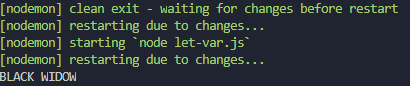
\includegraphics[width=15cm, height=1cm]{1.png}
  \end{center}
  este comando nos pedirá información adicional que podemos llenar a decisión de cada uno
    \begin{center}
    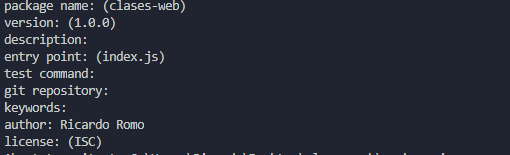
\includegraphics[width=15cm,height=5cm]{2.png}
  \end{center}
  Al ejecutar el comando, nos pedirá cierta información adicional dependiendo del programa que deseemos realizar, generando así nuestro archivo \textbf{package.json} con la lista de dependencias , módulos que queramos usar y la información introducida al inicializar npm .
  \lstinputlisting[firstline=1,lastline=11,style=htmlcssjs]{codigo/package.json} 
  Ahora necesitaremos el paquete \textbf{yargs} el cual te ayuda a crear herramientas interactivas de línea de comandos, analizando argumentos y generando una elegante interfaz de usuario.
  y para instalar como dependencia en nuestro package.json solo necesitaremos ingresar la siguiente línea de comandos en la terminal ubicada en nuestra carpeta:
  \begin{center}
    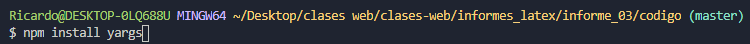
\includegraphics[width=15cm, height=1cm]{3.png}
  \end{center}
  Para confirmar la instalación podemos dirigirnos a nuestro \textbf{packege.json} y podemos observar que \textbf{yargs} ya se encuentra como una dependencia necesaria para nuestro programa 
  \lstinputlisting[firstline=7,lastline=13,style=htmlcssjs]{codigo/package.json} 
  Además de esto, podemos visualizar una nueva carpeta creada donde tendremos el módulo yargs.
  \begin{center}
    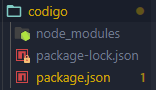
\includegraphics[width=5cm, height=3cm]{4.png}
  \end{center}

Ahora crearemos 3 carpetas:\\
\textbf{conf : } Almacenara las configuraciones dentro del yargs.
\textbf{controlador : }Realizara las actividades de crear, actualizar, borrar y listar las tareas.
\textbf{modelo : }En el cual se almacenara el .json con las tareas creadas.
\textbf{app.js : }que va ser el índex de nuestra aplicación.
\begin{center}
  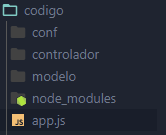
\includegraphics[width=5cm, height=3.5cm]{6.png}
\end{center}
    
Dentro de la carpeta \textbf{conf} crearemos un el documento yargs.js el cual tendrá las siguientes configuraciones.
\lstinputlisting[firstline=1,lastline=11,style=htmlcssjs]{codigo/conf/yars.js}
\begin{enumerate}
  \item declararemos dos objetos, uno llamado \textbf{description} y \textbf{complete} que almacenaran los siguientes atributos.
  \begin{enumerate}
    \item \textbf{demand :} Especifica que al recibir datos, este debe ser ingresado obligatoriamente.
    \item \textbf{alias :} Es una forma rápida de referirnos a este atributo para no llamarlo de forma completa.
    \item \textbf{desc: }Descripción de lo que realiza este objeto
    \item \textbf{default: }El valor que toma automáticamente si no es ingresado ningún dato.
  \end{enumerate}
\end{enumerate}

\textbf{Importar paquete yargs: }\\
Para importar nuestro paquete \textbf{yargs} previamente instalado declararemos una variable constante llamada argv, la cual almacenara las líneas de comando insertadas desde la terminal al llamar a nuestro índex.
\lstinputlisting[firstline=13,lastline=24,style=htmlcssjs]{codigo/conf/yars.js}
\begin{enumerate}
  \item \textbf{require() : }Es una función que nos permite incluir módulos ya instalados, y llamándolos solo con su nombre
  \item \textbf{command.() : } Define los comandos por los cuales se va a recibir la información, los atributos que recibe son:
  \item \begin{enumerate}
    \item Nombre por el cual se puede ingresar
    \item Descripción de las actividades que realiza
    \item Atributos propios de estos, en este caso sus atributos se encuentran en los objetos \textbf{description} y \textbf{complete} antes ya declarada.
  \end{enumerate}
  \item \textbf{.argv : } Obtenga los argumentos como un simple objeto.
\end{enumerate}

Al instanciar todo esto lo hacemos de manera local para el documento, es decir solo este documento podrá manejar nuestro \textbf{argv} por lo tanto tenemos que exportarlo para que otros documentos también la puedan utilizar.
\lstinputlisting[firstline=26,lastline=28,style=htmlcssjs]{codigo/conf/yars.js}
\begin{enumerate}
  \item \textbf{module.exports{}} especifica que objetos, variables, funciones van hacer exportadas para ser usadas.
\end{enumerate}

Ahora dentro de controlador crearemos un archivo llamado \textbf{task-for-do} el cual nos ayudara a crear, actualizar, borrar y listar las tareas.




Primero importamos el módulo \textbf{fs} que nos ayudara con el manejo de archivos (module de node js que por default ya está instalado) y creamos un array \textbf{taskfordo} el cual almacenara las tareas.
\lstinputlisting[firstline=1,lastline=3,style=htmlcssjs]{codigo/controlador/task-for-do.js}
Crearemos la carpeta modelo y dentro de este el archivo data.json en la cual se va almacenar.
\begin{center}
  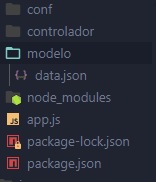
\includegraphics[width=3cm, height=4cm]{5.png}
\end{center} 

Dentro de \textbf{task\-for\-do.js} crearemos los métodos \textbf{load\_data()} (cargar data.json) y \textbf{save\_data}(Guardar en data.json)
\lstinputlisting[firstline=5,lastline=15,style=htmlcssjs]{codigo/controlador/task-for-do.js}
\begin{enumerate}
  \item \textbf{load\_data()}
  \begin{enumerate}
    \item almacena e nuestro vector \textbf{taskfordo} el archivo \textbf{data.json}  ingresando su ubicación.
  \end{enumerate}
  \item \textbf{sabe\_data()}
  \begin{enumerate}
    \item creamos una variable \textbf{data} el cual transforma los datos almacenados en \textbf{taskfordo} a un formato \textbf{JSON}
    \item \textbf{fs.writefile()} es una función de \textbf{fs} que nos permite crear un archivo enviando los parámetros de: 
    \begin{enumerate}
      \item Dirección donde se almacena y se encuentra el archivo
      \item Los datos que se almacenaran
      \item Funcion de error en caso de fallar con la operación.
    \end{enumerate}
  \end{enumerate}
\end{enumerate}

\textbf{Funcion Crear "create()"}

\lstinputlisting[firstline=17,lastline=26,style=htmlcssjs]{codigo/controlador/task-for-do.js}
\begin{enumerate}
  \item Definimos que esta función va a recibir un atributo llamado \textbf{description}
  \item Cargamos nuestro archivo data en el cual vamos almacenar con la función ya creada \textbf{load\_data()}
  \item Creamos una variable \textbf{task} que almacenara \textbf{description} y un atributo boleano llamado complete que identifica si la tarea esta completa.
\end{enumerate}

\textbf{Funcion Listar "getlist()"}
\lstinputlisting[firstline=28,lastline=31,style=htmlcssjs]{codigo/controlador/task-for-do.js}
\begin{enumerate}
  \item Cargamos nuestras tareas con \textbf{load\_data()} (esta carga \textbf{data.json} en la variable \textbf{taskfordo})
  \item Retornemos \textbf{taskfordo}
\end{enumerate}

\textbf{Función actualizar "update()"}
\lstinputlisting[firstline=33,lastline=43,style=htmlcssjs]{codigo/controlador/task-for-do.js}
\begin{enumerate}
  \item Definimos la función \textbf{update} la cual recibe los parámetros de la descripción, y el estado de completado.
  \item Cargamos en \textbf{taskfordo} nuestra \textbf{data.json} con la función \textbf{load\_data()}
  \item Declaramos una variable la cual almacena la posición dentro del vector \textbf{taskfordo} si este es igual a la descripción que recibe la función.
  \item Si el índice es encontrado remplazaremos el atributo complete por \textbf{true}  
  \item Guardaremos el cambio que hemos realizado con la funcion \textbf{save\_data()}
  \item y retornamos el valor \textbf{true} en caso de ser completado con éxito y si no el valor \textbf{false}
\end{enumerate}

\textbf{Función Eliminar "deleted()"}
\lstinputlisting[firstline=46,lastline=56,style=htmlcssjs]{codigo/controlador/task-for-do.js}
\begin{enumerate}
  \item Esta función recibirá el atributo de la descripción del atributo a eliminar.
  \item Cargamos nuestra data con la función \textbf{load\_data()}
  \item Identificamos la posición en la que se encuentra el elemento a eliminar
  \item Si se encuentra el índice utilizamos la función \textbf{-filter()} el cual almacena todo los datos que no contengan esa información
  \item Actualizamos nuestra variable \textbf{taskfordo} por el nuevo vector que se encuentra ya sin la tarea deseada.
  \item Utilizamos la función \textbf{save\_data()} para guardar los cambios.
  \item Retornamos un valor \textbf{true} si se completó con éxito, caso contrario un \textbf{false}.
\end{enumerate}

\textbf{Exportación de funciones}\\
\lstinputlisting[firstline=58,lastline=62,style=htmlcssjs]{codigo/controlador/task-for-do.js}
Al igual que yargs necesitamos exportar estas funciones para que nuestra \textbf{app.js} pueda usarlos para esto utilizaremos \textbf{module.exports{}}
\\
Ahora crearemos en la carpeta raíz nuestro \textbf{app.js} el cual va ser nuestro menú para usar cada una de nuestras funciones y utilizando \textbf{yargs} para poder ingresar los parámetros
\begin{center}
  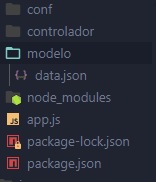
\includegraphics[width=3cm, height=4cm]{5.png}
\end{center} 

Dentro de \textbf{app.js :}
Importaremos nuestra configuración de \textbf{yargs.js} y nuestras funciones dentro de \textbf{task\-for\-do.js}.\\
Además instalaremos \textbf{colors} con el comando \textbf{npm install colors --save} dentro de nuestro \textbf{app.js}
\lstinputlisting[firstline=1,lastline=3,style=htmlcssjs]{codigo/app.js}
Iniciaremos una variable \textbf{command} que almacenara la lectura e ingreso de datos desde la terminal
\lstinputlisting[firstline=5,lastline=5,style=htmlcssjs]{codigo/app.js}

Para el menú utilizaremos un \textbf{switch/case} que nos permitirá ejecutar cualquiera de las opciones dependiendo el caso que se ingrese
\lstinputlisting[firstline=7,lastline=30,style=htmlcssjs]{codigo/app.js}
\begin{enumerate}
  \item \textbf{Create}
  \begin{enumerate}
    \item Creamos una variable \textbf{task}, la cual llama a la variable \textbf{tasks} que almacena nuestras funciones creadas en \textbf{task\-for\-do.js}
    \item llamamos a la función \textbf{create} y enviamos nuestro \textbf{argv.description} que está vinculado con la configuración de nuestro \textbf{yargs}  
    \item Mandamos a imprimir en consola las tareas que tenemos
  \end{enumerate}
  \item \textbf{List}
  \begin{enumerate}
    \item Creamos una variable llamada \textbf{list} que almacena nuestro \textbf{taskfordo} que nos lanza la función \textbf{getlist()} de nuestro archivo \textbf{task\-for\-do.js} almacenado en \textbf{tasks}
    \item Mandamos a imprimir con \textbf{color.} especificando el color que queremos que aparezca en pantalla.
  \end{enumerate}
  \item \textbf{Update}
  \begin{enumerate}
    \item Creamos una variable \textbf{resp} la cual llamara al método \textbf{update} y enviamos el nombre de la tarea a actualizar
  \end{enumerate}
  \item \textbf{Clean}
  \begin{enumerate}
    \item Creamos la variable \textbf{del} la cual almacena la respuesta del método \textbf{deleted} enviando el nombre de la tarea a eliminar
  \end{enumerate}
  \item \textbf{Default:} simplemente imprime en la consola en caso de que cualquier caso ingresado no se encuentre.
\end{enumerate}

\textbf{EJECUCIÓN}\\
Dirígete a terminal dentro de la carpeta raíz y ejecuta el comando \textbf{npm init} para iniciar y \textbf{npm install} para instalar las dependencias agregadas en \textbf{package.json} :
\begin{enumerate}
  \item \textbf{Crear Tareas}
  \begin{center}
    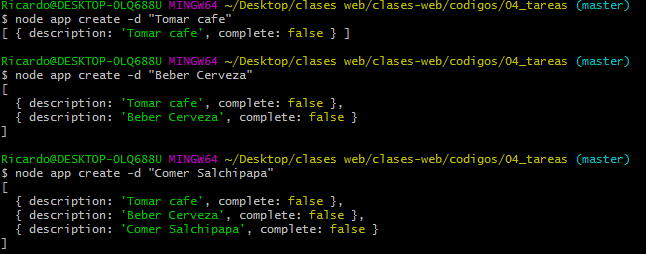
\includegraphics[width=15cm, height=7cm]{7.png}
  \end{center}
  \item \textbf{Listar tareas}
  \begin{center}
    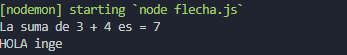
\includegraphics[width=15cm, height=5cm]{8.png}
  \end{center}
  \item \textbf{Actualizar tareas}
  \begin{center}
    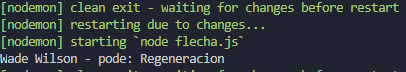
\includegraphics[width=15cm, height=7cm]{9.png}
  \end{center}
  \item \textbf{Eliminar tareas}
  \begin{center}
    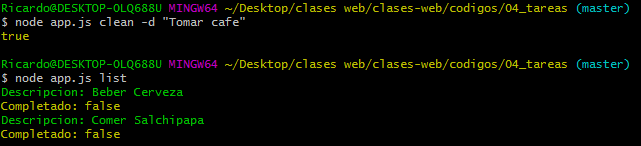
\includegraphics[width=15cm, height=7cm]{10.png}
  \end{center}

\end{enumerate}
\textbf{Este informe y código lo pudes encontrar aqui: } \url{https://github.com/rromom/clases-web.git}
\end{document}